\documentclass{standalone}
\usepackage[svgnames]{xcolor}
\usepackage{tikz}
\usepackage[english]{babel}
\usepackage[T1]{fontenc}
\usepackage[utf8]{inputenc}
\usepackage{microtype}

\tikzstyle{peers}=[draw,circle,black]
%,bottom color=DodgerBlue, top color= white,
\tikzstyle{pose}=[color=LawnGreen]
\tikzstyle{nege}=[color=FireBrick]
\tikzstyle{c1}=[fill=DodgerBlue]
\tikzstyle{c2}=[fill=OrangeRed]
\tikzstyle{c3}=[fill=SpringGreen]
\tikzstyle{disa}=[line width=4pt,dashed]
\tikzstyle{label}=[scale=0.8]
\begin{document}
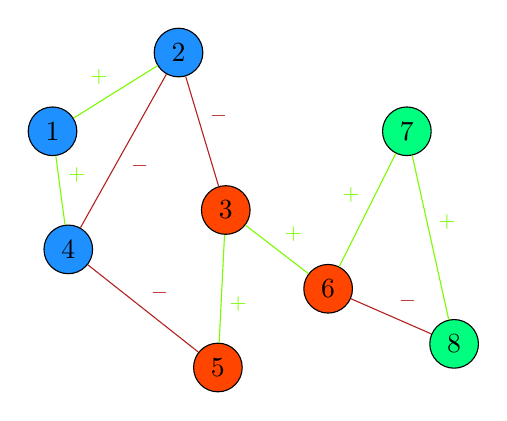
\begin{tikzpicture}[auto]
	% \foreach \place/\name in {%
	% {(0,4)/1}, {(1.6,5)/2}, {(0.2,2.5)/4},
	% {(2.2,3)/3}, {(2.1,1)/5}, {(3.5,2)/6},
	% {(4.5,4)/7}, {(5.1,1.3)/8}}
    % \node[peers] (\name) at \place {\name};
\foreach \place/\name in { {(0,4)/1}, {(1.6,5)/2}, {(0.2,2.5)/4}}
    \node[peers,c1] (\name) at \place {\name};
\foreach \place/\name in {{(2.2,3)/3}, {(2.1,1)/5}, {(3.5,2)/6}}
    \node[peers,c2] (\name) at \place {\name};
\foreach \place/\name in  {{(4.5,4)/7}, {(5.1,1.3)/8}}
    \node[peers,c3] (\name) at \place {\name};
	\foreach \source/\dest in {1/2, 1/4, 3/5, 3/6, 7/8}
  \draw[pose] (\source) edge node[label]{$+$} (\dest);

  \foreach \source/\dest in {2/3,4/5,6/8}
    \draw[nege] (\source) edge node[label]{$-$} (\dest);

	% \draw[pose,disa] (6) edge node[label]{$+$} (7);
	% \draw[nege,disa] (2) edge node[label]{$-$} (4);
	\draw[pose] (6) edge node[label]{$+$} (7);
	\draw[nege] (2) edge node[label]{$-$} (4);

\end{tikzpicture}
\end{document}

